\documentclass[]{article}
\usepackage{lmodern}
\usepackage{amssymb,amsmath}
\usepackage{ifxetex,ifluatex}
\usepackage{fixltx2e} % provides \textsubscript
\ifnum 0\ifxetex 1\fi\ifluatex 1\fi=0 % if pdftex
  \usepackage[T1]{fontenc}
  \usepackage[utf8]{inputenc}
\else % if luatex or xelatex
  \ifxetex
    \usepackage{mathspec}
  \else
    \usepackage{fontspec}
  \fi
  \defaultfontfeatures{Ligatures=TeX,Scale=MatchLowercase}
\fi
% use upquote if available, for straight quotes in verbatim environments
\IfFileExists{upquote.sty}{\usepackage{upquote}}{}
% use microtype if available
\IfFileExists{microtype.sty}{%
\usepackage{microtype}
\UseMicrotypeSet[protrusion]{basicmath} % disable protrusion for tt fonts
}{}
\usepackage[margin=1in]{geometry}
\usepackage{hyperref}
\PassOptionsToPackage{usenames,dvipsnames}{color} % color is loaded by hyperref
\hypersetup{unicode=true,
            pdftitle={README for the data preparation part},
            pdfauthor={Group 2},
            colorlinks=true,
            linkcolor=Maroon,
            citecolor=Blue,
            urlcolor=blue,
            breaklinks=true}
\urlstyle{same}  % don't use monospace font for urls
\usepackage{longtable,booktabs}
\usepackage{graphicx,grffile}
\makeatletter
\def\maxwidth{\ifdim\Gin@nat@width>\linewidth\linewidth\else\Gin@nat@width\fi}
\def\maxheight{\ifdim\Gin@nat@height>\textheight\textheight\else\Gin@nat@height\fi}
\makeatother
% Scale images if necessary, so that they will not overflow the page
% margins by default, and it is still possible to overwrite the defaults
% using explicit options in \includegraphics[width, height, ...]{}
\setkeys{Gin}{width=\maxwidth,height=\maxheight,keepaspectratio}
\IfFileExists{parskip.sty}{%
\usepackage{parskip}
}{% else
\setlength{\parindent}{0pt}
\setlength{\parskip}{6pt plus 2pt minus 1pt}
}
\setlength{\emergencystretch}{3em}  % prevent overfull lines
\providecommand{\tightlist}{%
  \setlength{\itemsep}{0pt}\setlength{\parskip}{0pt}}
\setcounter{secnumdepth}{0}
% Redefines (sub)paragraphs to behave more like sections
\ifx\paragraph\undefined\else
\let\oldparagraph\paragraph
\renewcommand{\paragraph}[1]{\oldparagraph{#1}\mbox{}}
\fi
\ifx\subparagraph\undefined\else
\let\oldsubparagraph\subparagraph
\renewcommand{\subparagraph}[1]{\oldsubparagraph{#1}\mbox{}}
\fi

%%% Use protect on footnotes to avoid problems with footnotes in titles
\let\rmarkdownfootnote\footnote%
\def\footnote{\protect\rmarkdownfootnote}

%%% Change title format to be more compact
\usepackage{titling}

% Create subtitle command for use in maketitle
\providecommand{\subtitle}[1]{
  \posttitle{
    \begin{center}\large#1\end{center}
    }
}

\setlength{\droptitle}{-2em}

  \title{README for the data preparation part}
    \pretitle{\vspace{\droptitle}\centering\huge}
  \posttitle{\par}
    \author{Group 2}
    \preauthor{\centering\large\emph}
  \postauthor{\par}
      \predate{\centering\large\emph}
  \postdate{\par}
    \date{\texttt{December,\ 2nd,\ 2019}}


\begin{document}
\maketitle
\begin{abstract}
This Chapter is describes the process from raw to clean data, as well as
the data sources. In other words it explains the scripts
`DataCleaning2.R' and `functionGetCleanClass2.R' and therefore also the
function `getCleanClass2'.
\end{abstract}

\hypertarget{description-of-the-goal}{%
\subsection{Description of the Goal}\label{description-of-the-goal}}

We want to predict wheter a college football Quarterback (QB), Running
Back (RB) or Wide Receiver (WR) will be drafted into the NFL or not. For
this purpose we try to combine data from different sources. This starts
with game data from College Football and will be extended with further
information like the NFL Combine or the Pro Day. Since we want to apply
supervised learning, we would also need a `Y', which contains the
information, if a player was drafted or not.

\hypertarget{data-source}{%
\subsection{Data Source}\label{data-source}}

Most of our data was uploaded some years ago to Kaggle
(\url{https://www.kaggle.com/mhixon/college-football-statistics}), but
has no relevant scprips that were made of it and try to predict the NFL
Draft. These Datasets contain much more information about college
football, than we would need. We only use following data sets for all
the years:

\begin{itemize}
\tightlist
\item
  player-game-statistics.csv

  \begin{itemize}
  \tightlist
  \item
    One observation in these files contains the information about one
    player in one game.
  \end{itemize}
\item
  player.csv

  \begin{itemize}
  \tightlist
  \item
    One observation in these files contains information about height,
    weight, schools etc. of one player
  \end{itemize}
\end{itemize}

The best data sets (in order of lenght) about the NFL Combine and the
Pro Day we found, is also one from Kaggle
(\url{https://www.kaggle.com/kbanta11/nfl-combine}). Unfortunately it
turned out that, compared to the College data, not even 10\% of the
players have accessible Combine/Pro Day data, which is why we took them
out again. Otherwise too many cells would contain NA and could not be
analized with all the algorithms we want to use.

The third data set we integrate, is from Pro Football reference
(\url{https://www.pro-football-reference.com/play-index/draft-finder.cgi?}).
It contains the information about the NFL Drafts from the last couple of
years. In terms of return on investment, the most reasonable option to
obtain the data, was to filter the Years 2005 to 2019, the positions QB,
WR, RB and then only keeping the Rows ``Year'', ``Rnd'', ``Pick'',
``Player'', ``Pos'', ``Tm'', ``College.Univ''. To reproduce it, this is
the way: set the named filters -\textgreater{} Get Results
-\textgreater{} Share \& More -\textgreater{} Modify \& Share table
-\textgreater{} remove all other Variables we don't need -\textgreater{}
comma-separated (in the yellow box) -\textgreater{} copy paste the data
into a new .txt file.

\hypertarget{the-data-cleaning-process}{%
\subsection{The data cleaning process}\label{the-data-cleaning-process}}

In order to clean the data fast and easy and with only a few manual
steps, we build a function, that will provide us the clean data sets in
the formate we want them to be. This function is called getCleanClass2
and is coded in the file `functionGetCleanClass2.R'.

\hypertarget{function-getcleanclass2}{%
\subsubsection{Function
`getCleanClass2'}\label{function-getcleanclass2}}

The function getCleanClass2 needs the inputs `draftyear' (just year
number), the player-game-statistics from the two years before the draft,
the player list of the two previous years (both from first source on
Kaggle) and the draft dataset (from the third source). Its output is a
table with the information about one single draft year. The following
explanations in plain text shall summarize the steps, if you desire more
details, please see the comments in the file `functionGetCleanClass2.R'.

getCleanClass2 will first drop all the variables, that are irrelevant
for QB, RB and WR and remove observations, that don't contain any
results in a game (e.g.~0's in every cell of a row). It adds a column
called `Games.Played', which allows to see, how many games were played
to reach the other results, that are summed up. After that, information
about the players is matched to the obtained data. Then the most
important column is matched; the target value called `Drafted', whicht
is 0 if a player is not drafted and 1 if he is. Unfortunately the
information about the draft is not available with the player code which
is used for matching before, which means that the match has to be done
by the name. This can result in some mistakes, which cannot be avoided.
Then duplicates non-matchable players as well as variables that are
available twice from matching are removed. After these steps, the
dataframe will contain four parts in every observation:

\begin{itemize}
\tightlist
\item
  Col 1 - 5: Information about the Player
\item
  Col 6: Our Y called `Drafted'
\item
  Col 7 - 30: The summed game statistics of the previous year
\item
  Col 31 - 54: The summed game statistics of two years prior to the
  draft
\end{itemize}

The next steps separate these parts and group the two years together, in
order to obtain a dataframe with 30 variables containing the game stats
of both years together. This has the advantage, that Players that could
only be matched to the year before the draft still can be analized.

\hypertarget{computing-the-clean-data}{%
\subsubsection{Computing the clean
data}\label{computing-the-clean-data}}

In the script `DataCleaning2.R' the function `getCleanClass2' is applied
to all the available years of data, to obtain a dataframe for every
year. In the last part, all these dataframes are rbind-ed together and
cleaned from duplicates. This overall precedure allows us to obtain all
eligable players on the first hand and than only keep the latest
information about players that played a senior year (those who have been
drafted in their junior year will appear with their junior year).

\hypertarget{validation-of-the-data-and-further-cleaning}{%
\subsubsection{Validation of the Data and further
cleaning}\label{validation-of-the-data-and-further-cleaning}}

Just by having a look at the different rows (=players) can already help
to see wheter the data seems to be right or not. Most of the data seems
to be plausible, but for example the QB Jimmy Garoppolo has not his
total performance in our data.

\begin{longtable}[]{@{}lrrrrrr@{}}
\caption{Comparison of Jimmy Garoppolo's performance}\tabularnewline
\toprule
& Drafted & Pass.Att & Pass.Comp & Pass.Yards & Pass.TD &
Games.Played\tabularnewline
\midrule
\endfirsthead
\toprule
& Drafted & Pass.Att & Pass.Comp & Pass.Yards & Pass.TD &
Games.Played\tabularnewline
\midrule
\endhead
Our Data & 1 & 127 & 80 & 1036 & 10 & 3\tabularnewline
Wikipedia & 1 & 1108 & 706 & 8873 & 84 & 26\tabularnewline
\bottomrule
\end{longtable}

Unfortunately, the missing 23 games could not be found anywhere in the
input data, which means, that there must be some errors in the data. An
other way to look at this issue is by looking at the histograms of
``Games.Played'' of all players and compare it to the histogram of the
drafted ones.
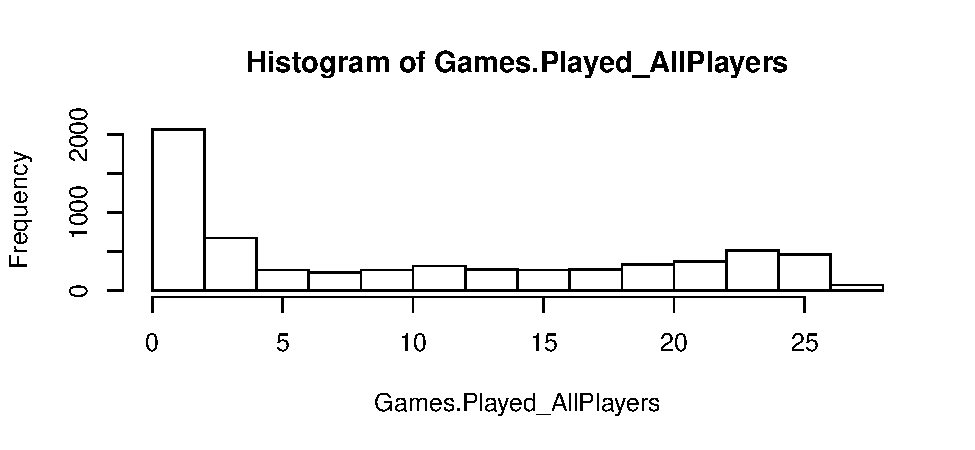
\includegraphics{RM_DataHandling_files/figure-latex/unnamed-chunk-3-1.pdf}
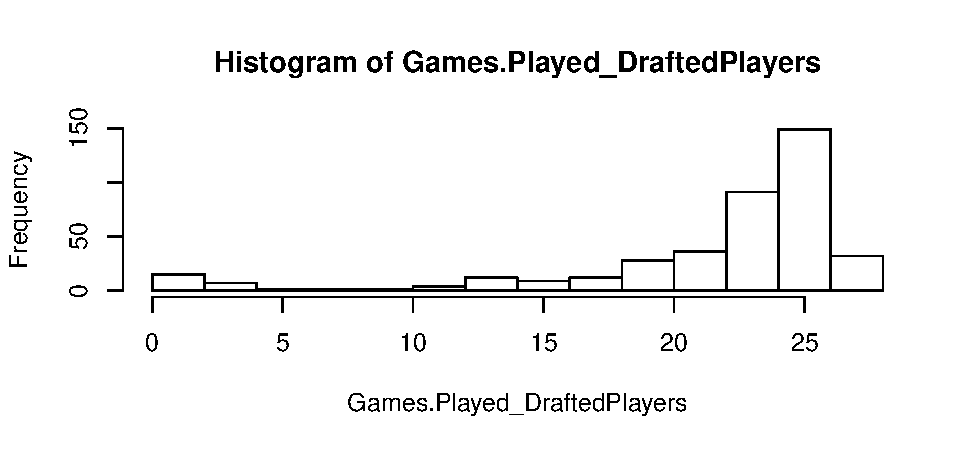
\includegraphics{RM_DataHandling_files/figure-latex/unnamed-chunk-3-2.pdf}

As we see in the histograms, there is a majority of players that played
less than 5 games (at least according to our data) and some of them have
been drafted. It seems very unlikely, that a player is drafted if he
played less than 5 games in the two seasons prior to the draft.
Therefore it is very likely, that all the drafted players with less than
5 played games are mistakes. As we see in the second histogram, there
were no players drafted haveing played between 5 and 9 games. Looking at
our business case, we decided to eliminate all players with less than 10
played games in the data. This eliminates the errors and players, that a
priori don't have a chance to be drafted. The new data frame is called
`CleanClass2007to2014\_3.Rdata'.

\hypertarget{sampling-the-data}{%
\subsubsection{Sampling the data}\label{sampling-the-data}}

Because our target value is distributed very inequally (see table
below), we applied 4 different sampling methods, to approach this issue.
The methods are called `oversampling', `undersampling', `rose both' and
`smote'. We then cross-validate the different data in all the models, to
find the best data to use for training the optimal model.

\begin{longtable}[]{@{}lrl@{}}
\caption{Number of observations and Ratio of Drafted Players in the
Dataframes}\tabularnewline
\toprule
& Observations & Drafted\_Ratio\tabularnewline
\midrule
\endfirsthead
\toprule
& Observations & Drafted\_Ratio\tabularnewline
\midrule
\endhead
Before filter & 6372 & 06.24\%\tabularnewline
No Sampling & 3008 & 12.43\%\tabularnewline
Oversampling & 4022 & 50.00\%\tabularnewline
Undersampling & 654 & 50.00\%\tabularnewline
Rose Both & 2338 & 50.81\%\tabularnewline
Smote & 4221 & 52.35\%\tabularnewline
\bottomrule
\end{longtable}

As we see, applying the filter Games.played \textgreater= 10 already
decreases the inequality of drafted vs.~undrafted players by dismissing
players with a chance of being drafted close to zero or have errors in
the data. By sampling the data we can make the distribution close to
fifty/fifty, but if this will really improve our predictions needs to be
cross-validated with the models. Since the filter shall dismiss the
errors, we only continue with the filtered data (one set unsampled and
four sampled).

\hypertarget{the-clean-data}{%
\subsection{The clean data}\label{the-clean-data}}

After all the described processes the five dataframes (one unsampled and
four sampled) contain following variables:

\begin{itemize}
\tightlist
\item
  Player.Code: A unique Number for matching the data
\item
  Name: Name of the Player
\item
  Class: A factor showing the college year the player was in when being
  in draft class with levels:

  \begin{itemize}
  \tightlist
  \item
    JR=Junior (3.year)
  \item
    SR=Senior (4.year)
  \end{itemize}
\item
  Position: A factor with Position of the Player (filtered for only
  QB=Quarterback, RB=Runningback, WR=Wide Receiver)
\item
  Year: Shows the year the player was in the draft class
\item
  Drafted: The targe which is 1 when a player was drafted and 0 when a
  player was not drafted
\item
  Rush.Att: Summed rushing attempts over both seasons (mainly for RB)
\item
  Rush.Yard: Summed rushing yards over both seasons (mainly for RB)
\item
  Rush.TD: Summed rushing TD over both seasons (mainly for RB)
\item
  Pass.Att: Summed passing attempts over both seasons (mainly for QB)
\item
  Pass.Comp: Summed passing completions over both seasons (mainly for
  QB)
\item
  Pass.Yard: Summed passing yards over both seasons (mainly for QB)
\item
  Pass.TD: Summed passing TD over both seasons (mainly for QB)
\item
  Pass.Int: Summed Inteceptions thrown over both seasons (mainly for QB)
\item
  Pass.Conv: Summed thrown 2-pt conversion over both seasons (mainly for
  QB)
\item
  Rec: Summed receptions over both seasons (mainly for WR)
\item
  Rec.Yards: Summed reception yards over both seasons (mainly for WR)
\item
  Rec.TD: Summed reception TD over both seasons (mainly for WR)
\item
  Kickoff.Ret: Summed Kickoff returns over both seasons (mainly for
  WR/RB)
\item
  Kickoff.Ret.Yard: Summed Kickoff return yards over both seasons
  (mainly for WR/RB)
\item
  Kickoff.Ret.TD: Summed Kickoff return TD over both seasons (mainly for
  WR/RB)
\item
  Punt.Ret: Summed punt returns over both seasons (mainly for WR/RB)
\item
  Punt.Ret.Yard: Summed punt return yards over both seasons (mainly for
  WR/RB)
\item
  Punt.Ret.TD: Summed punt return TD over both seasons (mainly for
  WR/RB)
\item
  Off.2XP.Att: Summed 2 point conversion attempts over both seasons
\item
  Off.2XP.Made: Summed 2 point conversions made over both seasons
\item
  Safety: Being tackeled in the own end zone summed over both seasons(=2
  pt for opponent)
\item
  Fumble: Dropped balls summed over both seasons
\item
  Fumble.Lost: Dropped balls recovered by opponent summed over both
  seasons
\item
  Games.Played: Number of games played over both seasons (filter
  applied: \textgreater= 10)
\end{itemize}

\hypertarget{for-the-documentation}{%
\section{For the Documentation:}\label{for-the-documentation}}

For further details on this part, please see `RM\_DataHandling.pdf'.

\hypertarget{data-source-1}{%
\subsection{Data Source}\label{data-source-1}}

Most of our data was uploaded some years ago to Kaggle
(\url{https://www.kaggle.com/mhixon/college-football-statistics}), but
has no relevant scprips that were made of it and try to predict the NFL
Draft. These Datasets contain much more information about college
football, than we would need.

The best data sets (in order of lenght) about the NFL Combine and the
Pro Day we found, is also one from Kaggle
(\url{https://www.kaggle.com/kbanta11/nfl-combine}). Unfortunately it
turned out that, compared to the College data, not even 10\% of the
players have accessible Combine/Pro Day data, which is why we took them
out again. Otherwise too many cells would contain NA and could not be
analized with all the algorithms we want to use.

The third data set we integrate, is from Pro Football reference
(\url{https://www.pro-football-reference.com/play-index/draft-finder.cgi?}).
It contains the information about the NFL Drafts from the last couple of
years.

\hypertarget{the-data-cleaning-process-1}{%
\subsection{The data cleaning
process}\label{the-data-cleaning-process-1}}

In order to clean the data fast and easy and with only a few manual
steps, we build a function, that will provide us the clean data sets in
the formate we want them to be. This function is called getCleanClass2
and is coded in the file `functionGetCleanClass2.R'. After putting them
together and removing duplicates, we apply a filter on the games a
player played, in order to remove observations containing errors
(details explained in `RM\_DataHandling.pdf').

\hypertarget{sampling-the-data-1}{%
\subsection{Sampling the data}\label{sampling-the-data-1}}

Because our target value is distributed very inequally (see table
below), we applied 4 different sampling methods, to approach this issue.
The methods are called `oversampling', `undersampling', `rose both' and
`smote'. We then cross-validate the different data in all the models, to
find the best data to use for training the optimal model.

\begin{longtable}[]{@{}lrl@{}}
\caption{Number of observations and Ratio of Drafted Players in the
Dataframes}\tabularnewline
\toprule
& Observations & Drafted\_Ratio\tabularnewline
\midrule
\endfirsthead
\toprule
& Observations & Drafted\_Ratio\tabularnewline
\midrule
\endhead
Before filter & 6372 & 06.24\%\tabularnewline
No Sampling & 3008 & 12.43\%\tabularnewline
Oversampling & 4022 & 50.00\%\tabularnewline
Undersampling & 654 & 50.00\%\tabularnewline
Rose Both & 2338 & 50.81\%\tabularnewline
Smote & 4221 & 52.35\%\tabularnewline
\bottomrule
\end{longtable}

As we see, applying the filter Games.played \textgreater= 10 already
decreases the inequality of drafted vs.~undrafted players by dismissing
players with a chance of being drafted close to zero or have errors in
the data. By sampling the data we can make the distribution close to
fifty/fifty, but if this will really improve our predictions needs to be
cross-validated with the models. Since the filter shall dismiss the
errors, we only continue with the filtered data (one set unsampled and
four sampled).


\end{document}
